\documentclass[20pt,]{extarticle}
\usepackage[margin=0.6in]{geometry}
\pagenumbering{gobble}
\usepackage{lmodern}
\usepackage{amssymb,amsmath}
\usepackage{ifxetex,ifluatex}
\usepackage{fixltx2e} % provides \textsubscript
\ifnum 0\ifxetex 1\fi\ifluatex 1\fi=0 % if pdftex
  \usepackage[T1]{fontenc}
  \usepackage[utf8]{inputenc}
\else % if luatex or xelatex
  \ifxetex
    \usepackage{mathspec}
  \else
    \usepackage{fontspec}
  \fi
  \defaultfontfeatures{Ligatures=TeX,Scale=MatchLowercase}
\fi
% use upquote if available, for straight quotes in verbatim environments
\IfFileExists{upquote.sty}{\usepackage{upquote}}{}
% use microtype if available
\IfFileExists{microtype.sty}{%
\usepackage{microtype}
\UseMicrotypeSet[protrusion]{basicmath} % disable protrusion for tt fonts
}{}
\usepackage{hyperref}
\PassOptionsToPackage{usenames,dvipsnames}{color} % color is loaded by hyperref
\hypersetup{unicode=true,
            pdftitle={Introduction to Locality-Sensitive Hashes},
            pdfauthor={Tyler Neylon},
            colorlinks=true,
            linkcolor=black,
            citecolor=Blue,
            urlcolor=Blue,
            breaklinks=true}
\urlstyle{same}  % don't use monospace font for urls
\usepackage{graphicx,grffile}
\makeatletter
\def\maxwidth{\ifdim\Gin@nat@width>\linewidth\linewidth\else\Gin@nat@width\fi}
\def\maxheight{\ifdim\Gin@nat@height>\textheight\textheight\else\Gin@nat@height\fi}
\makeatother
% Scale images if necessary, so that they will not overflow the page
% margins by default, and it is still possible to overwrite the defaults
% using explicit options in \includegraphics[width, height, ...]{}
\setkeys{Gin}{width=\maxwidth,height=\maxheight,keepaspectratio}
\IfFileExists{parskip.sty}{%
\usepackage{parskip}
}{% else
\setlength{\parindent}{0pt}
\setlength{\parskip}{6pt plus 2pt minus 1pt}
}
\setlength{\emergencystretch}{3em}  % prevent overfull lines
\providecommand{\tightlist}{%
  \setlength{\itemsep}{0pt}\setlength{\parskip}{0pt}}
\setcounter{secnumdepth}{5}
% Redefines (sub)paragraphs to behave more like sections
\ifx\paragraph\undefined\else
\let\oldparagraph\paragraph
\renewcommand{\paragraph}[1]{\oldparagraph{#1}\mbox{}}
\fi
\ifx\subparagraph\undefined\else
\let\oldsubparagraph\subparagraph
\renewcommand{\subparagraph}[1]{\oldsubparagraph{#1}\mbox{}}
\fi
\usepackage{subfig}
\AtBeginDocument{%
\renewcommand*\figurename{Figure}
\renewcommand*\tablename{Table}
}
\AtBeginDocument{%
\renewcommand*\listfigurename{List of Figures}
\renewcommand*\listtablename{List of Tables}
}
\usepackage{float}
\floatstyle{ruled}
\makeatletter
\@ifundefined{c@chapter}{\newfloat{codelisting}{h}{lop}}{\newfloat{codelisting}{h}{lop}[chapter]}
\makeatother
\floatname{codelisting}{Listing}
\newcommand*\listoflistings{\listof{codelisting}{List of Listings}}

\title{Introduction to Locality-Sensitive Hashes}
\author{Tyler Neylon}
\date{145.2018}

% Begin custom, non-pandoc commands.

\newcommand{\latexonlyrule}{\rule}
\newenvironment{densearray}{\begin{array}{rcl}}{\end{array}}
\newcommand{\class}[1]{}
\newcommand{\Rule}[3]{}
\newcommand{\optquad}{\quad}
\newcommand{\smallscrneg}{}
\newcommand{\smallscr}[1]{}
\newcommand{\bigscr}[1]{#1}
\newcommand{\smallscrskip}[1]{}

% End custom, non-pandoc commands.

\begin{document}
\maketitle

CHECK:

\begin{itemize}
\tightlist
\item
  Update images to all use unitRadius = 2 (or consider it)
\item
  I think figure 4 only has 3 hashes and the text says 4 Try updating it
  to really have 4 hashes, but I can fall back to 3 if 4 looks bad.
\item
  Search this file for all instances of CHECK, IMAGE, XXX
\item
  Check that the two pdf versions look good, including cross-references
\item
  Check that the references header has no number
\item
  Try to nicify the images in the pdf files
\item
  Ensure that all references to figures in the text are done by
  mentioning a figure number.
\item
  Follow-up ideas (put these somewhere centralized with other Unbox post
  ideas)
\item
  MinHash
\item
  ProxHash
\item
  The J-L Lemma
\end{itemize}

\newcommand{\R}{\mathbb{R}}
\newcommand{\Z}{\mathbb{Z}}
\newcommand{\eqnset}[1]{\left.\mbox{$#1$}\;\;\right\rbrace\class{postbrace}{ }}
\providecommand{\optquad}{\class{optquad}{}}
\providecommand{\smallscrneg}{\class{smallscrneg}{ }}
\providecommand{\bigscr}[1]{\class{bigscr}{#1}}
\providecommand{\smallscr}[1]{\class{smallscr}{#1}}
\providecommand{\smallscrskip}[1]{\class{smallscrskip}{\hskip #1}}

\emph{Locality-sensitive hashes} are techniques that dramatically speed
up search-for-neighbors or near-duplication detection on data. They can
be used, for example, to filter out duplicates of scraped web pages at
an impressive speed, or to perform near-constant-time lookups of nearby
points from a geospatial data set.

When you think about hash functions, you might think about \emph{hash
tables}, which is perhaps the most common use case. As a reminder, the
hash functions used in a hash table are designed to map a data structure
to an integer that can be used to look in a particular \emph{bucket}
within the hash table to retrieve (or delete) that element. Common
containers with string keys like JavaScript object attributes and Python
dictionaries are based on hash tables. Although they might not
\emph{guarantee} constant-time lookups, in practice they effectively
provide them. Hash functions used for hash tables are called
\emph{universal hash functions}. {[}CHECK{]}

There are a number of other classes of hash functions as well. For
example the SHA1 cryptographic hash function is designed to be
\emph{difficult to reverse}, which is useful if you want to store
someone's password as a hashed value. {[}CHECK{]} Another
security-oriented hash function is CHECK, which is actually designed to
be \emph{expensive to compute}, as this can deter malicious
ne'er-do-wells from easily building large lookup tables to be able to
reverse a hash on more likely input values. Hash functions like these
are called \emph{secure hash functions}. {[}CHECK{]}

Here are what all these various hash functions have in common:

\begin{itemize}
\tightlist
\item
  They map a wide variety of input data types to discrete values.
\item
  In practice, we care about whether or not two (or more) input values
  map to the same output (hashed) value.
\end{itemize}

Locality-sensitive hash (LSH) functions are specifically designed so
that collisions of the hash value are \emph{more likely} given two input
values that are \emph{close together}. Just as there are different
implementations of secure hash functions for different use cases, there
are different implementations of LSH functions for different data types
and for different definitions of being \emph{close together}. In this
post, I'll give a brief overview of the key ideas, and take a look at a
toy example based on \emph{random projections} of vectors into
lower-dimensional spaces.

\section{An example}\label{an-example}

It will probably be much easier to grasp the main idea with an example.
(The ``toy example'' for random projections will come later. This is
like a mini-toy example.)

Suppose you have a million people from across the United States all
standing in a huge room. It's your job to get people who live close
together to stand together in groups. Imagine how much time it would
take to walk up to each person, ask for their street address, map that
to a lat/long pair, then write some code to find reasonable geographic
clusters, and walk up to every person again and tell them their cluster
number. It's a disaster.

Here's a much better way to solve this problem: Write every U.S. zip
code on poster boards, and hang those from the ceiling. Then announce to
everyone to go stand under the zip code where they live.

Voila! That's much easier, right? The main idea here is also the main
idea behind locality-sensitive hashes. We're taking an arbitrary data
type (a person, who we could of as a ton of data including their street
address), and mapping that data into a set of discrete values (zip
codes) such that people who live close together probably hash to the
same value. In other words, the clusters are very likely to be groups of
neighbors.

The distinction between walking sequentially up to each person versus
parallelizing the work by asking everyone to find their own way to their
zip code was not an accident. Besides avoiding whatever clustering
algorithm you'd have to run on lat/long coordinates, another advantage
of this hashing approach is that it's extremely friendly to parallel
processing. Despite caring about \emph{relationships} within your data,
you can still split up the data any way you like and compute the hashes
in a fully parallelized fashion.

Another property of this example is that it is \emph{approximate} in the
sense that some people may live across the street from each other, but
happen to cross a zip code line, in which case they would not be
clustered together here. As we'll see below, it's also possible for data
points to be clustered together even when they're very far apart,
although a well-designed LSH can at least give some mathematical
evidence that this will be a rare event, and some implementations manage
to guarantee certain bad cases (such as clustering of very far points or
non-clustering of very close points) never happen.

\section{Hashing points via
projection}\label{hashing-points-via-projection}

Let's start with an incredibly simple mathematical function that we can
treat as an LSH. Define \(f:\R^2 \to \Z\) for a point \(x\in\R^2\) by

\[ f(x) := \lfloor x_1 \rfloor; \]

that is \(f(x)\) is the largest integer \(a\) for which \(a\le x_1.\)
(For example, \(f((3.2, -1.2)) = 3.\))

Let's suppose we choose points at random by uniformly sampling from the
origin-centered circle \(\mathcal C\) with radius 3:

\[ \mathcal C := \{ (x, y) : x^2 + y^2 \le 3^2 \}. \]

If we want to find which of our points in \(\mathcal C\) are close
together, we can estimate this relationship by clustering together
points \(a\) and \(b \in \mathcal C\) iff (if and only if)
\(f(a) = f(b).\) It will be handy to introduce the notation \(a \sim b\)
to indicate that \(a\) and \(b\) are in the same cluster. With that
notation, we can write our current hash setup as

\[ a \sim b \iff h_1(a) = h_1(b). \]

Figure~\ref{fig:fig1} shows an example of such a clustering.

\begin{figure}
\centering
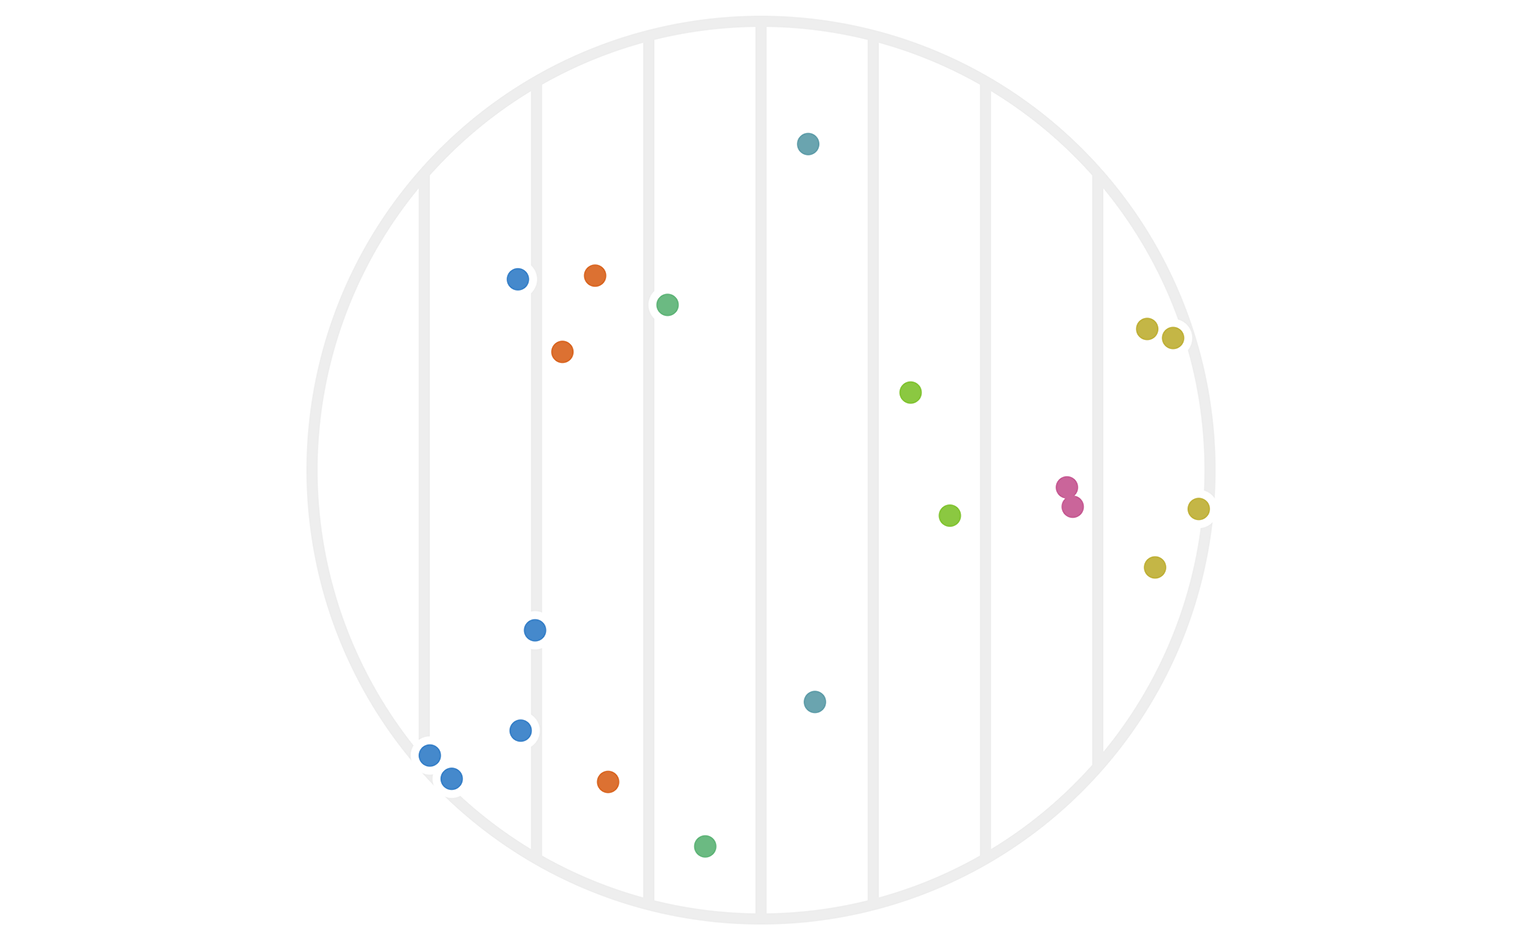
\includegraphics{images/lsh_image1_v2.png}
\caption{Twenty points chosen randomly in a circle with radius 4. Each
point \(x\) is colored based on its hash value
\(h_1(x).\)}\label{fig:fig1}
\end{figure}

You can immediately see that some points are far apart yet clustered,
while others are relatively close yet unclustered. There's also a sense
that this particular hash function \(h_1\) was arbitrarily chosen to
focus on the x-axis. What would have happened with the same data if we
had used instead \(h_2(x) := \lfloor x_2 \rfloor?\) The result is
figure~\ref{fig:fig2}.

\begin{figure}
\centering
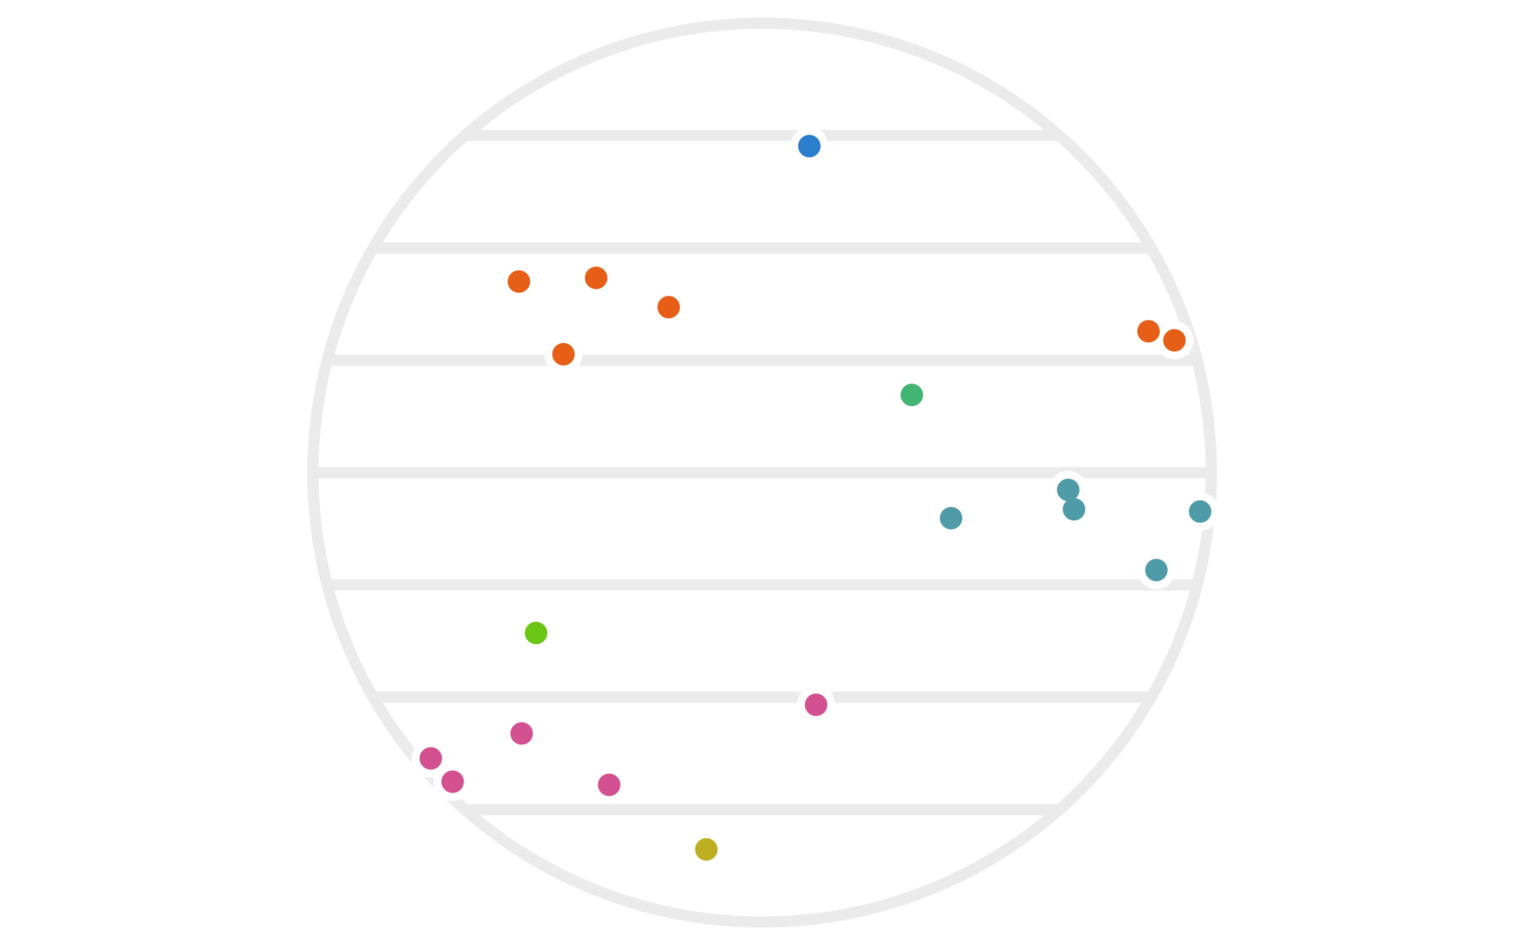
\includegraphics{images/lsh_image2.png}
\caption{The same twenty points as figure 1, except that we're using the
\(y\) values (instead of \(x\) values) to determine the hash-based
cluster colors this time around.}\label{fig:fig2}
\end{figure}

While neither clustering alone is amazing, things start to work better
if we use both of them simultaneously. That is, we can redefine our
clustering via

\begin{equation} a \sim b \iff h_1(a) = h_1(b) \text{ and } h_2(a) = h_2(b). \label{eq:eq1}\end{equation}

Our same example points are shown under this new clustering in
figure~\ref{fig:fig3}.

\begin{figure}
\centering
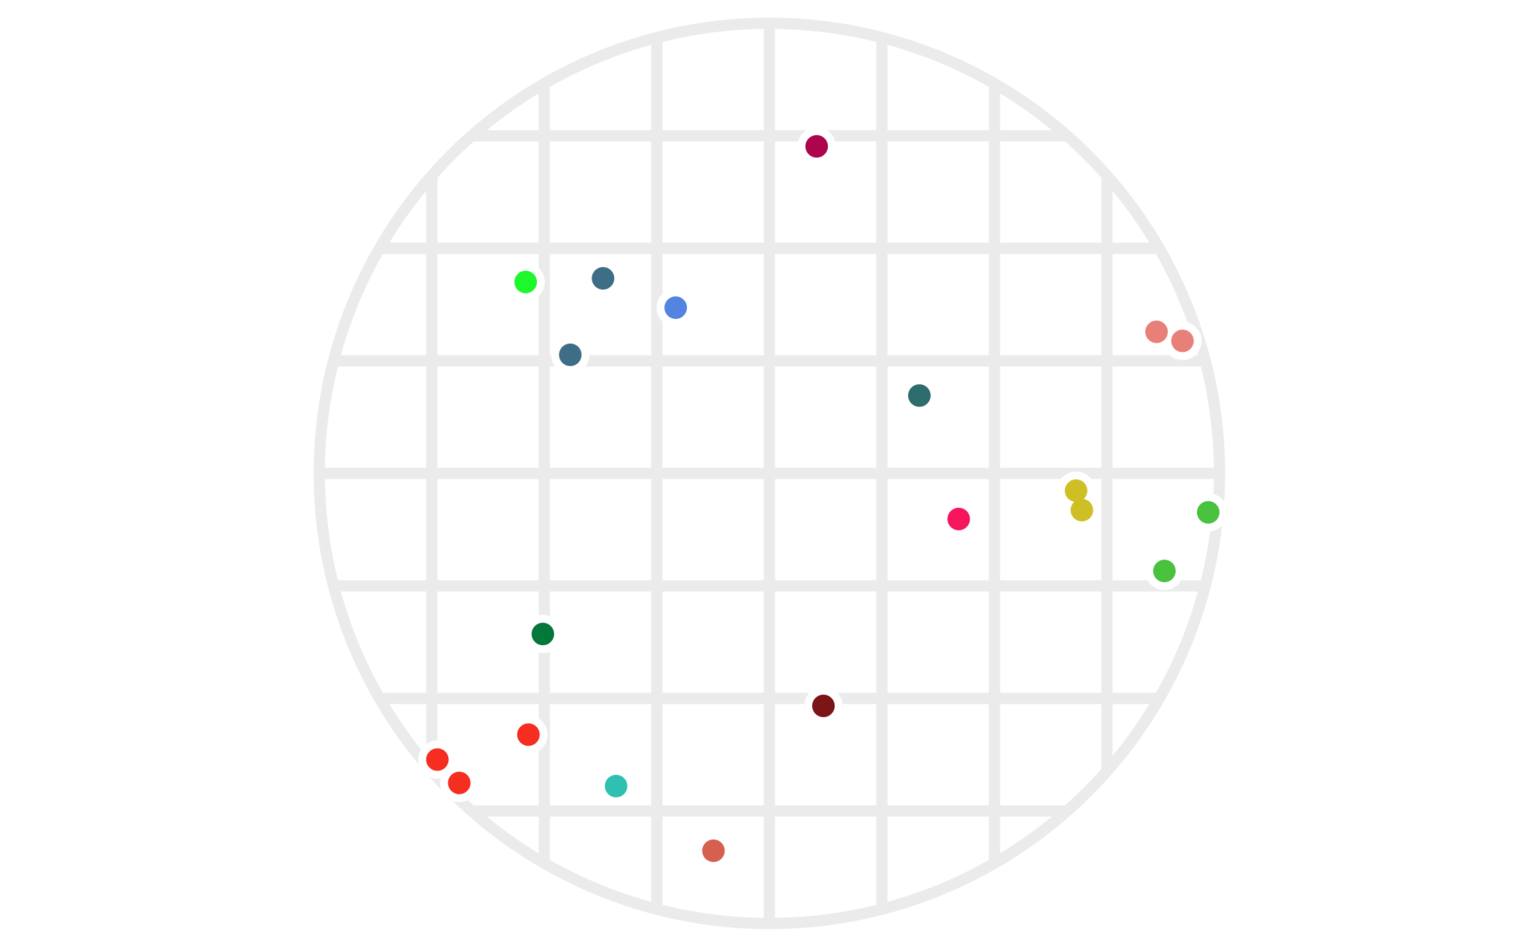
\includegraphics{images/lsh_image3.png}
\caption{The same twenty points clustered via two different hashes ---
one using \(\lfloor x\rfloor\), the other using \(\lfloor y\rfloor.\) As
before, points are colored based on which cluster they're in; a cluster
is the set of all points who share both their \(\lfloor x\rfloor\) and
their \(\lfloor y\rfloor\) values.}\label{fig:fig3}
\end{figure}

This does a much better job of avoiding clusters with points far apart,
although, as we'll see below, we can still make some improvements.

\subsection{Randomizing our hashes}\label{randomizing-our-hashes}

So far we've defined deterministic hash functions. Let's change that by
choosing a random rotation matrix \(U\) (a rotation around the origin)
along with a random offset \(b \in [0, 1).\) Given such a random \(U\)
and \(b,\) we could define a new hash function via

\[ h(x) := \lfloor (Ux)_1 + b \rfloor, \]

where I'm using the notation \(( \textit{vec} )_1\) to indicate the
first coordinate of the vector value \emph{vec} (that is, the notation
\((Ux)_1\) means the first coordinate of the vector \(Ux\)).

It may seem a tad arbitrary to use only the first coordinate here rather
than any other, but the fact that we're taking a random rotation first
means that we have the same set of possibilities, with the same
probability distribution, as we would when pulling out any other single
coordinate value.

The advantage of using randomized hash functions is that any theoretical
properties we want to discuss will apply without having to worry about
pathologically weird data. Conceptually, if we were using deterministic
hash functions, then someone could choose the worst-case data for our
hash function, and we'd be stuck with that poor performance (for
example, choosing maximally-far apart points that are still clustered
together by our \(h_1\) function above). By using randomly chosen hash
functions, we can ensure that any average-case behavior of our hash
functions applies equally well to \emph{all data}. This same perspective
is useful for hash tables in the form of \emph{universal hashing}; if
randomized hash functions are a new idea for you, I recommend checking
out \href{https://en.wikipedia.org/wiki/Universal_hashing}{Wikipedia's
universal hashing page}.

Let's revisit the example points we used above, but now apply some
randomized hash functions. In figure CHECK, points are clustered iff
both of their hash values (from \(h_1()\) and \(h_2()\)) collide. We'll
use that same idea, but this time choose four rotations
\(U_1, \ldots, U_4\) as well as four offsets \(b_1, \ldots, b_4\) to
define \(h_1(), \ldots, h_4()\) via

\begin{equation} h_i(x) := \lfloor (U_i x)_1 + b_i \rfloor. \label{eq:eq3}\end{equation}

Figure~\ref{fig:fig4} shows the resulting clustering. This time, there
are 100 points since using more hash functions has effectively made the
cluster areas smaller (so we need higher point density to see points
that are clustered together now).

\begin{figure}
\centering
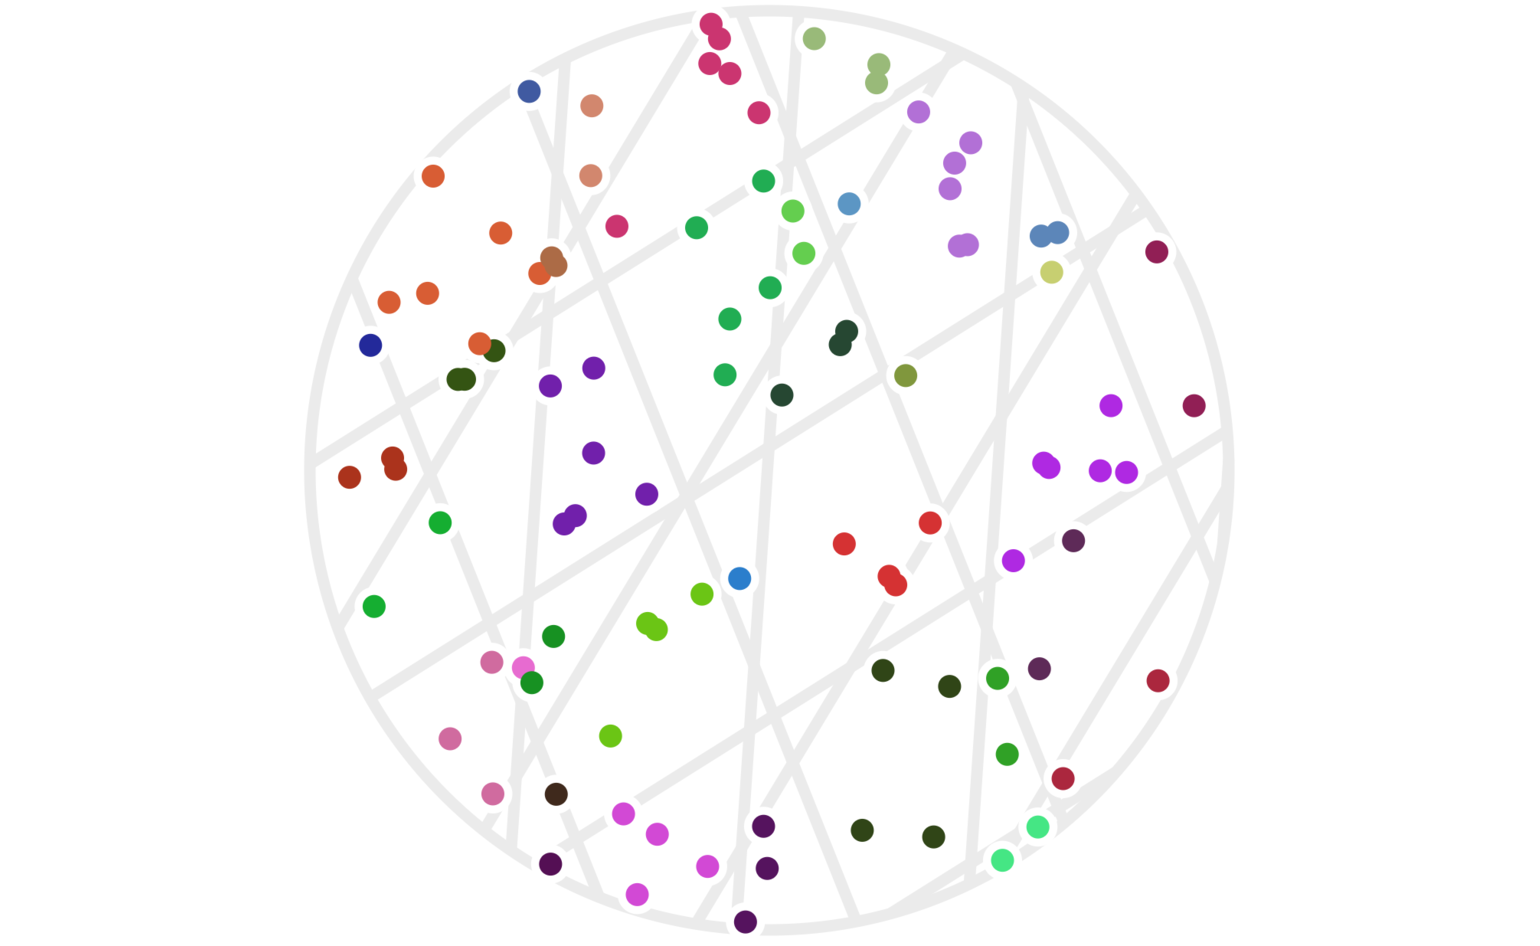
\includegraphics{images/lsh_image4.png}
\caption{One hundred random points clustered using four random hash
functions as defined by (\ref{eq:eq3}). Points have the same color when
all four of their hash values are the same. Each set of parallel light
gray lines delineates the regions with the same hash value for each of
the \(h_i()\) functions.}\label{fig:fig4}
\end{figure}

It's not obvious that we actually want to use all four of our hash
functions. The issue is that our clusters have become quite small. There
are a couple ways to address this. One is to simply increase the scale
of the hash functions; for example:

\[ \tilde h_i(x) := h_i(x/s), \]

where \(s\) is a scale factor (larger \(s\) values will result in larger
clusters).

However, there is something a bit more nuanced we can look at, which is
to allow some adaptability in terms of \emph{how many hash collisions we
require}. In other words, suppose we have \(k\) total hash functions
(just above, we had \(k=4\)). Instead of insisting that all \(k\) hash
values must match before we say two points are in the same cluster, we
could look at cases where some number \(j \le k\) of them matches. To
state this mathematically, we would rewrite equation (\ref{eq:eq1}) as

\begin{equation} a \sim b \iff \#\{i: h_i(a) = h_i(b)\} \ge j. \label{eq:eq2}\end{equation}

Something interesting happens here, which is that the \(a \sim b\)
relationship is no longer a clustering, but becomes more like adjacency
(that is, sharing an edge) in a graph. The difference is that, in a
clustering, if \(a\sim b\) and \(b\sim c,\) the we must have \(a\sim c\)
as well; this is called being \emph{transitively closed}. Graphs don't
need to have this property, and in our case as well, it's no longer true
that our similarity relationship is transitively closed.

It may help your intuition to see this new definition of \(a\sim b\) in
action on the same 100 points from figure~\ref{fig:fig4}. This time
(figure~\ref{fig:fig5}) there are twenty random hashes, and we're seeing
the graphs generated by (\ref{eq:eq2}) using cutoff values (values of
\(j\)) of 6, 7, 8, and 9. In other words, the top-left graph in
figure~\ref{fig:fig5} has an edge drawn between two points \(a\) and
\(b\) whenever there are at least 6 hash functions \(h_i()\) with
\(h_i(a) = h_i(b),\) out of a possible 20 used hash functions.

\begin{figure}
\centering
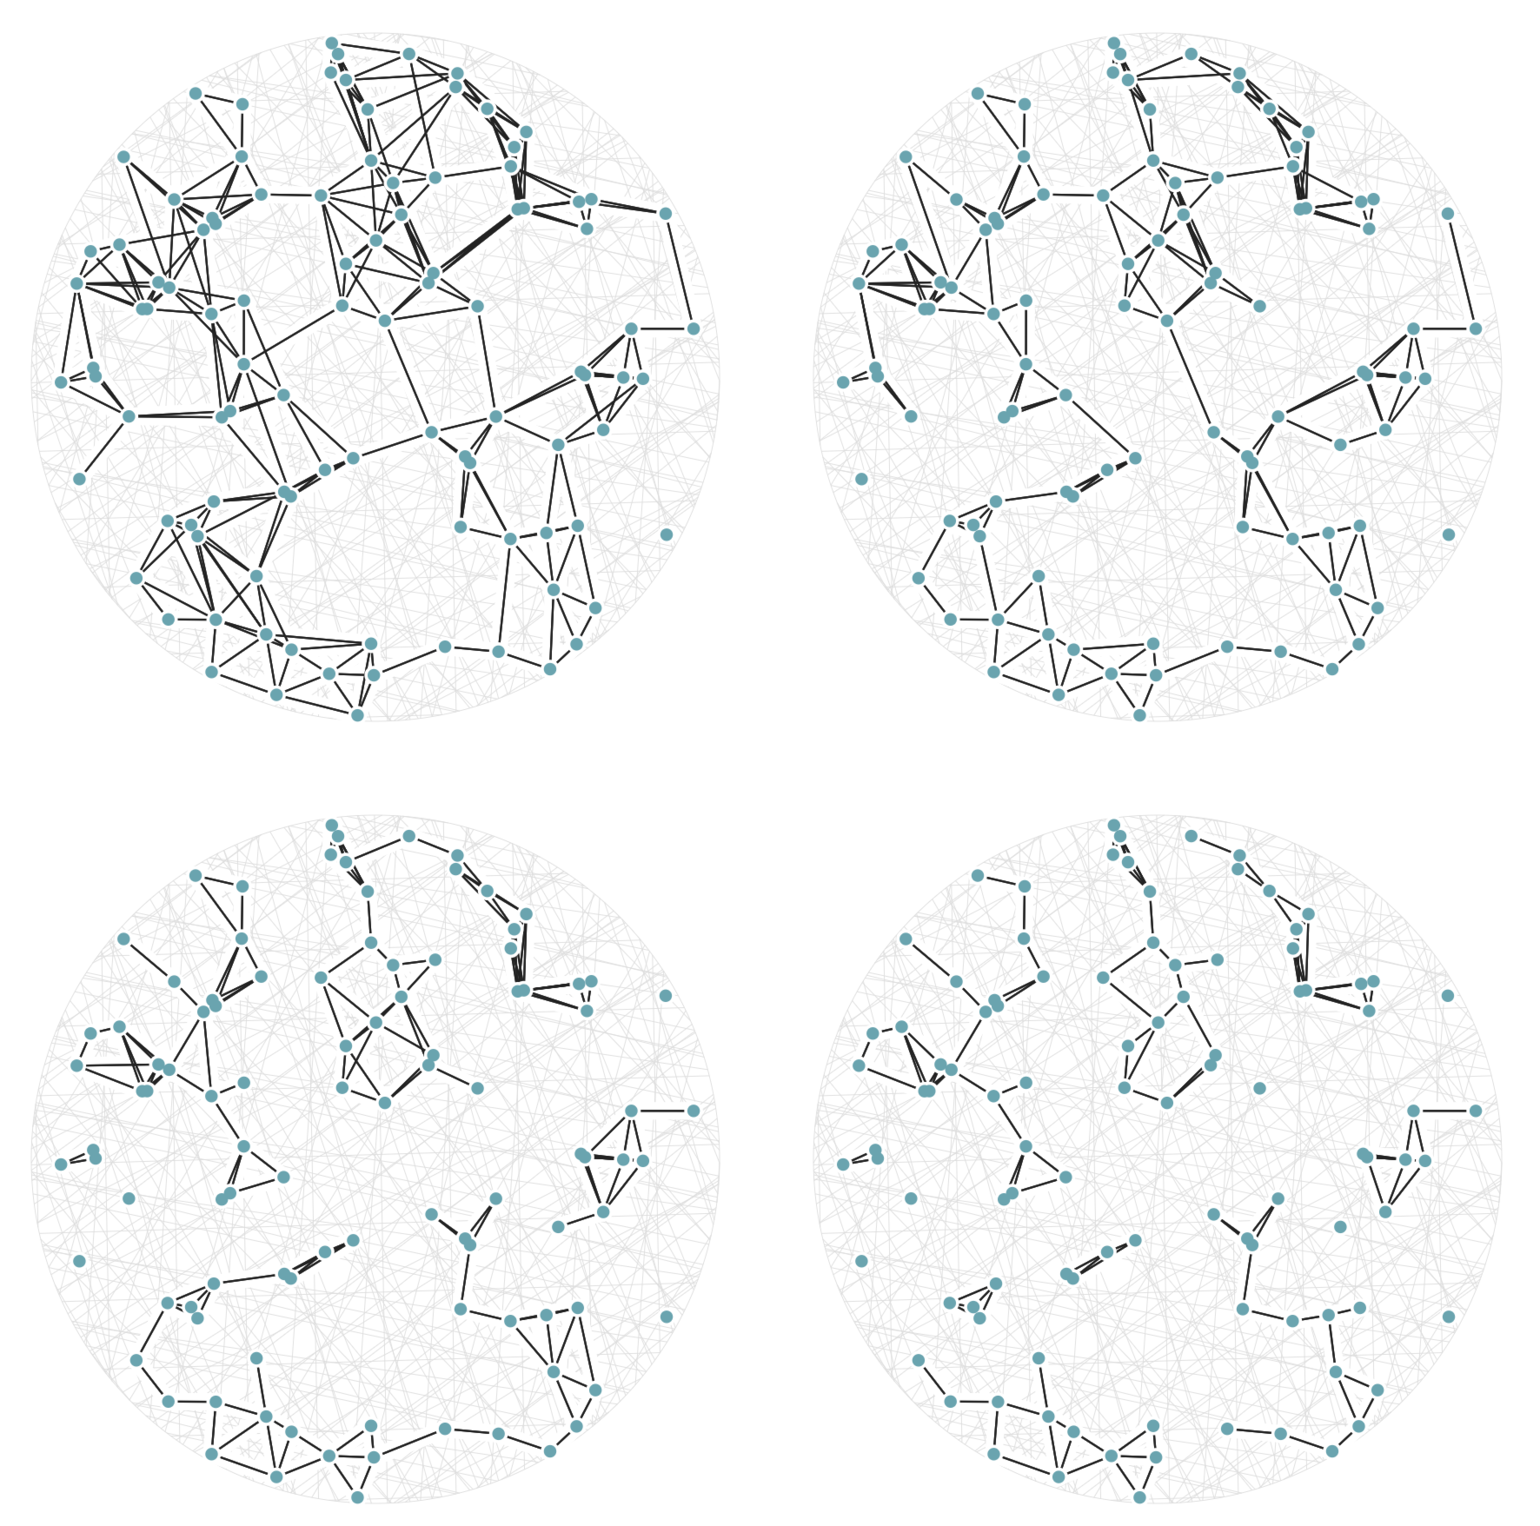
\includegraphics{images/lsh_image5.png}
\caption{A set of 100 random points with graph edges drawn according to
(\ref{eq:eq2}). There are 20 random hash functions used. The top-left
graph uses the cutoff value \(j=6.\) The remaining three graphs have
cutoff values \(j=7,\) 8, and 9; this means each graph is a subgraph
(having a subset of the edges) of the previous one.}\label{fig:fig5}
\end{figure}

In fact, we can visualize all possible cutoff values (values of \(j\) in
(\ref{eq:eq2})) of 6 or higher in a single image by using weighted
edges, like so: CHECK finish that sentence; explain why we start at 6

\begin{figure}
\centering
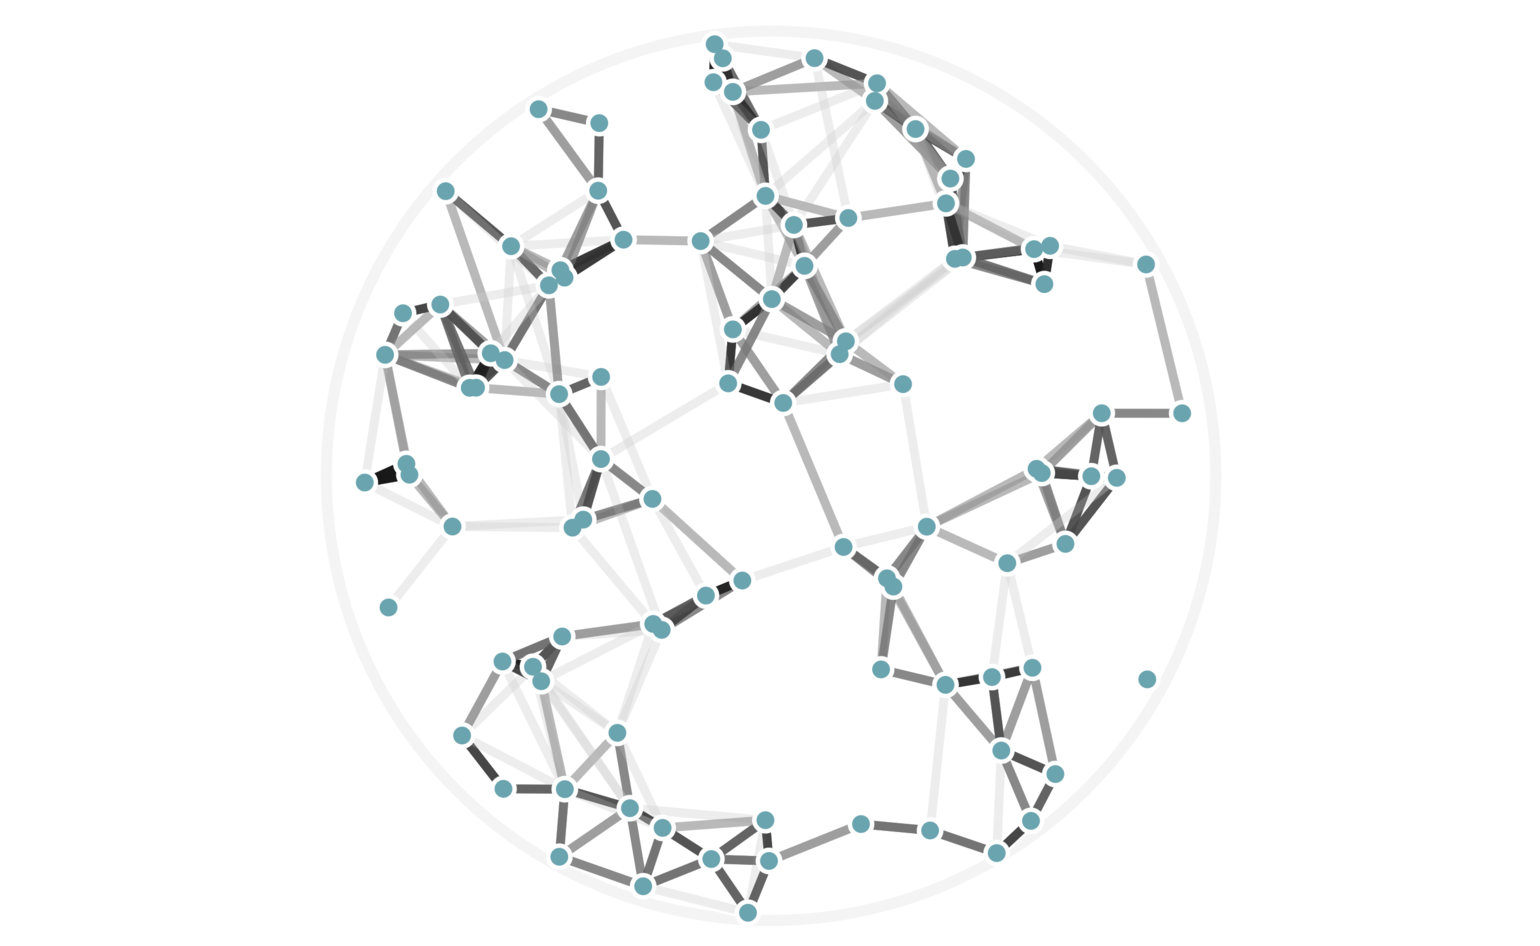
\includegraphics{images/lsh_image6.png}
\caption{description}
\end{figure}

Yet another fun way to get an intuitive feel for how much information
we're getting from our hashes is to see which subsets of our circle are
matched --- and to what degree --- by a given point:

IMAGE 8

{[}CHECK text on turning this into a graph{]}

\begin{figure}
\centering
\includegraphics{images/image8b@2x.gif}
\caption{Description}
\end{figure}

\subsection{Why this is faster}\label{why-this-is-faster}

So far we've been sticking to 2-dimensional data because that's easier
to visualize in an article. However, if you think about computing 10
hashes for every 2-dimensional point in order to find neighbors, it may
feel like you're doing more work than the simple solution of a linear
search through your points. Let's review cases where using an LSH is
more efficient than other methods of finding nearby points.

\subsubsection{Zero linear search}\label{zero-linear-search}

If you have a huge number \(n\) of points, and it's reasonable for you
to index those points ahead of time --- meaning, you can afford to
compute all \(k\) hash values for each point --- then you can completely
avoid the linear-time cost of a brute force search for nearby points
given a new query point. This speed-up is relevant in any dimension,
including the simple 2-dimensional case.

\subsubsection{Fewer hashes needed in higher
dimensions}\label{fewer-hashes-needed-in-higher-dimensions}

Another effect that may be less obvious is that you can get away with
fewer hash values (a smaller \(k\) value) in higher dimensions. There
are some mathematically sophisticated ways to quantify that statement,
but it may be even easier to understand graph based on empirically
derived data.

Here's a summary of some random sampling I did in order to explore the
relationship between various values of \(j\) for \(d=100\) dimensional
data using \(k=10\) different random hashes: CHECK

IMAGE 9

CHECK the whole next paragraph What's interesting here is that we get a
relatively tight box plot for \(j\) values around CHECK. This means that
we can choose the threshold \(j=CHECK\) in equation (\ref{eq:eq2}) and
have fairly good confidence that our hash-based ``nearby'' relationship
closely matches reality.

We can even quantify this precisely. Although this article doesn't
\emph{prove} the following implications, the empirical evidence found
CHECK(add link to code) strongly suggests that these are in fact the
correct values:

\[ \text{dist}(a, b) > \alpha \Rightarrow P(\#\{i : h_i(a) = h_i(b)\} < j) > 0.95; \]

\[ \text{dist}(a, b) < \beta  \Rightarrow P(\#\{i : h_i(a) = h_i(b)\} \ge j) < 0.05. \]

CHECK(the actual identities may end up being based on the left side
using a \(j\) value rather than a distance to start with).

We might interpret these last two expressions as saying that we believe
at least 99\% of our pairwise relationships are correctly classified.
And we're able to do so while saving about \(O(n)\) speed.

\subsection{Other data types and
approaches}\label{other-data-types-and-approaches}

This article has focused on numeric, 2-dimensional data because it's
easier to visualize. Locality-sensitive hashes can certainly be used for
many other data types, including strings, sets, or high-dimensional
vectors.

There are also other ways to specifically measure the performance of a
particular hashing approach. For example, CHECK.

Yet another ingredient to throw into the mix here are techniques to
boost performance which can treat any LSH as a black box. My favorite
approach here is to simply perform multiple lookups on a hash system,
each time using \(q + \varepsilon\) as an input, where \(q\) is your
query value, and \(\varepsilon\) is a random variable centered at zero.
CHECK(add a bit about what this achieves; add a reference for it)

There's a lot more that can be said about LSH techniques. If there is
reader interest, I may write a follow-up article explaining the details
of min-wise hashing, which is a fun case that's simultaneously good at
quickly finding nearby sets as well as nearby strings.

CHECK ensure that the references section is not numbered

\begin{center}\rule{0.5\linewidth}{\linethickness}\end{center}

\section{References}\label{references}

\end{document}
